%
% Acta Acustica united with Acustica -- Instructions for Authors, 2017-03-01
%
\documentclass[twocolumn]{article}

%%%%%%%%%%%%%%%%%%%%%%%%%%%%%%%%%%%%%%%%%%%%%%%
%% Comment / uncomment for one or two column(s) fomat
%\documentclass{article}

\usepackage[modulo,switch]{lineno}
\modulolinenumbers[1]
%%%%%%%%%%%%%%%%%%%%%%%%%%%%%%%%%%%%%%%%%%%%%%%
%% Comment / uncomment for showing line numbers
 \linenumbers

\usepackage[utf8]{inputenc}
\usepackage{amsmath}
\usepackage{amssymb}
\usepackage{float}
\usepackage{graphicx}
\usepackage{algorithm}
\usepackage[noend]{algpseudocode}

\makeatletter\@ifundefined{date}{}{\date{}}
\makeatother

%\markright{\hfill Kergomard {\em et al.}, p.\ }
\pagestyle{myheadings}

\paperheight297mm \paperwidth210mm
\textwidth170mm  \textheight245mm  \oddsidemargin 20mm
\evensidemargin\oddsidemargin \hoffset-22.4mm \voffset-28.4mm
\topmargin0pt \headheight20mm \headsep4mm \topskip0mm
\footskip17.5mm \columnsep7mm \arraycolsep2pt \parindent10pt
\renewcommand{\abstractname}{Introduction}

\DeclareMathSymbol{\sminus}{\mathbin}{AMSa}{"39}

\begin{document}

\title{TTT4180 Technical Acoustics - Assignment 7}

\author{Nicholas Bresina, Department of Electronic Systems, NTNU Trondheim, Norway \\
nicholdb@stud.ntnu.no}

\maketitle\thispagestyle{empty}

\begin{abstract}
This assignment in the Technical Acoustics course (TTT4180) revolves around
the transmission-line matrix (TLM) simulation technique used for acoustic waves
and studying a variety of acoustic wave propagation scenarios by simulation.

The report is split into two parts, where the first part provides a brief
description of methods used for an own implementation of TLM simulation in Python.
After, some results are presented and discussed, which were generated from said
implementation.

The second part contains further analyisis of sound pressure
with respect to distance, surface reflections, and the effect of a noise screen
on the sound pressure level.
Instead of using the own implementation, this part uses a given Matlab implementation
called TLMfig.

Lastly, the report gives a brief outlook with a discussion of difficulties
encountered during this assignment and final conclusions.
% Possibly add difficulties and gained knowledge
\end{abstract}


\section{Wave Propagation in a 2D Pipe}
To analyze the propagation of a wave in a pipe a 2D TLM implementation was needed.
Python was chosen, as it provides all of the necessary features in libraries such
as Numpy \cite{NumpyManual} for arrays and linear algebra and Matplotlib \cite{Matplotlib}
for plotting the results.

\subsection{Methods}
\subsubsection{TLM}
The implementation is strongly based on the article provided with the assignment
that describes TLM \cite{KagawaTLM}.
Nevertheless the most significant parts will be described in this section.

The main idea is to replace the continuous space with a grid of so-called nodes,
as shown in Fig. \ref{fig_tlm_mesh}.

\begin{figure}[H]
    \centering
    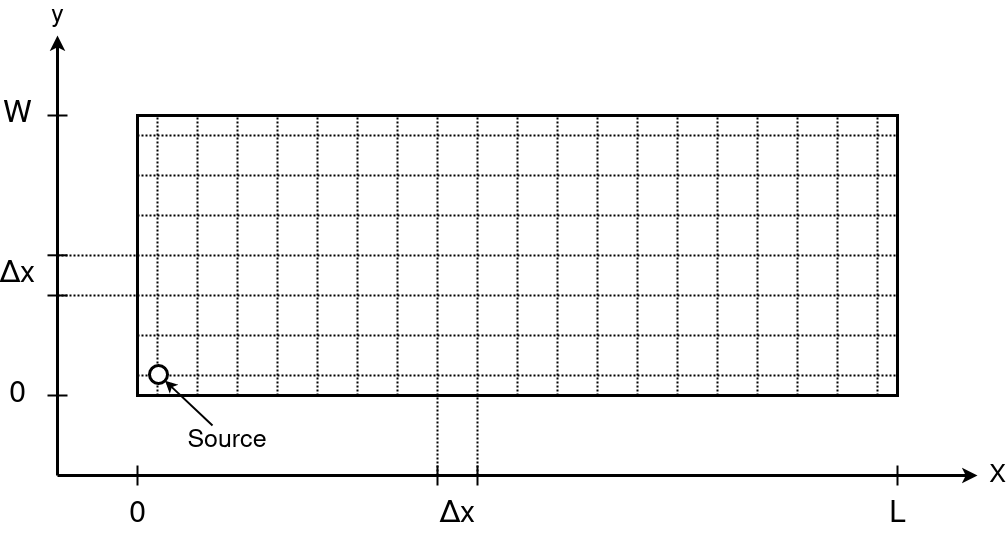
\includegraphics[width=75mm]{./Images/tlm_pipe.png}
    \caption{Example for TLM mesh placed on a pipe with dimensions L$\times$W}
    \label{fig_tlm_mesh}
\end{figure}

Each node can be represented as a pipe system with four branches.
And the nodes will be indexed with $i, j$ referencing their position on the grid.
Each branch will contain a superposition of an incident and scattering pressure waves.
These are denoted as $_{k}I_{i,j}^{n}$ and $_{k}S_{i,j}^{n}$ respectively, where
$k$ is the iteration count and $n$ is the branch index as shown in Fig.
\ref{fig_tlm_node}.

\begin{figure}[H]
    \centering
    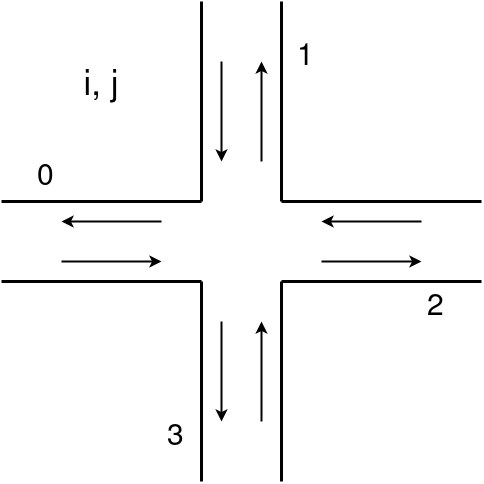
\includegraphics[width=50mm]{./Images/tlm_node.png}
    \caption{TLM node showing incident and outgoing waves as well as branch indexing}
    \label{fig_tlm_node}
\end{figure}

The incident waves of iteration $k$ will be turned into the scattering waves of
iteration $k+1$.
This can be written as

\begin{equation}
\begin{aligned}
    _{k+1}S_{i,j}^{0} &= \frac{1}{2}\left[\sminus_kI_{i,j}^{0}+_kI_{i,j}^{1}+_kI_{i,j}^{2}+_kI_{i,j}^{3}\right] \\
    _{k+1}S_{i,j}^{1} &= \frac{1}{2}\left[_kI_{i,j}^{0}-_kI_{i,j}^{1}+_kI_{i,j}^{2}+_kI_{i,j}^{3}\right] \\
    _{k+1}S_{i,j}^{2} &= \frac{1}{2}\left[_kI_{i,j}^{0}+_kI_{i,j}^{1}-_kI_{i,j}^{2}+_kI_{i,j}^{3}\right] \\
    _{k+1}S_{i,j}^{3} &= \frac{1}{2}\left[_kI_{i,j}^{0}+_kI_{i,j}^{1}+_kI_{i,j}^{2}-_kI_{i,j}^{3}\right] \\
\end{aligned}
\end{equation}

Which can be rewritten using the \textit{scattering matrix} as follows

\begin{equation}
\begin{bmatrix}
    _{k+1}S_{i,j}^{0} \\
    _{k+1}S_{i,j}^{1} \\
    _{k+1}S_{i,j}^{2} \\
    _{k+1}S_{i,j}^{3} \\
\end{bmatrix}
=
\frac{1}{2}
\begin{bmatrix}
    \sminus1 & 1 & 1 & 1 \\
    1 & \sminus1 & 1 & 1 \\
    1 & 1 & \sminus1 & 1 \\
    1 & 1 & 1 & \sminus1 \\
\end{bmatrix}
\begin{bmatrix}
    _kI_{i,j}^{0} \\
    _kI_{i,j}^{1} \\
    _kI_{i,j}^{2} \\
    _kI_{i,j}^{3} \\
\end{bmatrix}
\label{eq_scattering_matrix}
\end{equation}

The factor $\frac{1}{2}$ is due to the fact that we're considering the propagation of pressure waves.
An incident wave will evenly distribute the energy over the four branches, resulting
in a factor of $\frac{1}{4}$ with respect to the energy.
Given
\begin{equation}
    W_p = \frac{p_{rms}^{2}}{4K},
\end{equation}
which shows the square relationship between energy and pressure.
We can establish that a factor $\frac{1}{4}$ in energy to be a factor of $\frac{1}{2}$ with respect to
pressure.


The incident waves of the next iteration are the scattering waves of the respective
branches of the neighboring branches, which is shown in Fig. \ref{fig_tlm_nodes_transmission}.

\begin{figure}[H]
    \centering
    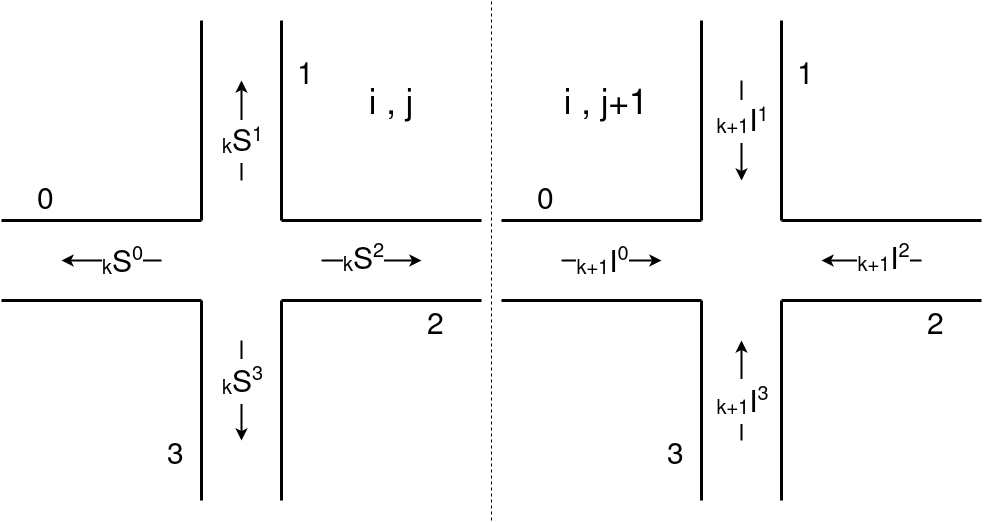
\includegraphics[width=75mm]{./Images/tlm_nodes_transmission.png}
    \caption{TLM nodes depicting the propagation of the scattering wave of branch $2$ to the incident wave of branch $0$ for the next iteration}
    \label{fig_tlm_nodes_transmission}
\end{figure}

Mathematically this can be written with the following equations

\begin{equation}
\begin{aligned}
    _{k+1}I_{i,j}^{0} &= _{k}S_{i,j\sminus 1}^{2} \\
    _{k+1}I_{i,j}^{1} &= _{k}S_{i,j\sminus 1}^{3} \\
    _{k+1}I_{i,j}^{2} &= _{k}S_{i,j+1}^{0} \\
    _{k+1}I_{i,j}^{3} &= _{k}S_{i,j+1}^{1} \\
\end{aligned}
\label{eq_propagation}
\end{equation}

Now these relations only count for all the nodes, that are not part of any of the boundaries.
At the boundary the next iteration's incident wave is given by the branch's current
scattering wave and the boundary's reflection coefficient $R_{m}$.

\begin{equation}
    _{k+1}I_{i,j}^{n} = R_{m}\cdot _{k}S_{i,j}^{n}
    \label{eq_boundary_propagation}
\end{equation}

The pressure can then be calculated by the superposition of all the waves in the node,
as given with

\begin{equation}
    _{k}p_{i,j} = \sum_{i=0}^{3} {}_kI_{i,j}^{n} - \sum_{i=0}^{3} {}_kS_{i,j}^{n}
\end{equation}

\subsubsection{Python Implementation}
In the Python code the nodes are represented as an array.
Where the size of the array is given by the physical dimensions L$\times$W and
the requirement to $\Delta x$, shown in Fig. \ref{fig_tlm_mesh}, which is

\begin{equation}
    \Delta x \leq \frac{\lambda_{max}}{10}
    \label{eq_delta_x}
\end{equation}

Where $\lambda_{max}$ is the wavelength of the maximum frequency that should be possible
to represented in the model, which is given by

\begin{equation}
    \lambda_{max} = \frac{c}{f_{max}}
    \label{eq_max_wavelength}
\end{equation}


The size of the arrays $M\times N$ is then calculated by
\begin{equation}
\begin{aligned}
    M &= ceil\left(\frac{\text{L}}{\Delta x}\right) \\
    N &= ceil\left(\frac{\text{W}}{\Delta x}\right) \\
\end{aligned}
\label{eq_integer_dimension}
\end{equation}

Because a wave propagates the distance $\Delta x$ in one iteration of the simulation,
this also gives the timestep with

\begin{equation}
    \Delta t = \frac{\Delta x}{c}
    \label{eq_delta_t}
\end{equation}

The easiest way to represent the different branches and differentiate between incident
and scattering wave is by using a multidimensional array.
The first two dimensions are the spatial integer dimensions $M\times N$.
The third dimension is used to stack one grid per branch for each incident and scattering
waves, as shown in Fig. \ref{fig_python_layers}.
An additional layer is added in the third dimension to represent source amplitudes placed
on the grid, which are written as $_{k}G_{i,j}$.
So the resulting array has the shape $\left(M, N, 9\right)$.

\begin{figure}[H]
    \centering
    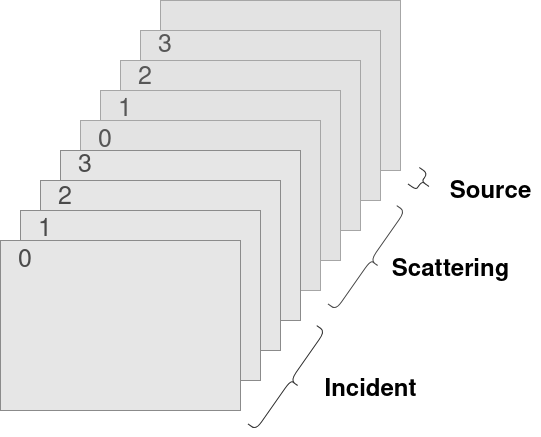
\includegraphics[width=75mm]{./Images/python_layers_bw.png}
    \caption{Depiction of the layers used in the implementation}
    \label{fig_python_layers}
\end{figure}

To have efficient computation two of these multidimensional arrays are being used,
where one corresponds to the current step and the other to the next iteration.
With that the values can easily be updated without generating temporary objects.
The full shape of the array is then given with $\left(M, N, 9, 2\right)$.

Eq. \ref{eq_scattering_matrix} has to be rewritten to allow incorporating the
mentioned source layer.

\begin{equation}
\begin{bmatrix}
    _{k+1}S_{i,j}^{0} \\
    _{k+1}S_{i,j}^{1} \\
    _{k+1}S_{i,j}^{2} \\
    _{k+1}S_{i,j}^{3} \\
\end{bmatrix}
=
\frac{1}{2}
\begin{bmatrix}
    \sminus1 & 1 & 1 & 1 & 1\\
    1 & \sminus1 & 1 & 1 & 1\\
    1 & 1 & \sminus1 & 1 & 1\\
    1 & 1 & 1 & \sminus1 & 1\\
\end{bmatrix}
\begin{bmatrix}
    _kI_{i,j}^{0} \\
    _kI_{i,j}^{1} \\
    _kI_{i,j}^{2} \\
    _kI_{i,j}^{3} \\
    _{k+1}G_{i,j} \\
\end{bmatrix}
\label{eq_source_scattering_matrix}
\end{equation}

Which will add the sources' amplitudes to the corresponding scattering waves.

Updating the incident waves can be done as described in the TLM chapter.

Using a feature of NumPy that allows matrix multiplication for multidimensional
arrays, it's possible to compute all scattering values using the \textit{scattering matrix}
for a whole $\left(M, 1\right)$ or $\left(1, N\right)$ vector at once.
Updating the incident waves can also be achieved with one iteration in each the x-direction
and the y-direction, updating the horizontal and vertical propagation respectively.
This approach allows reducing the run time complexity to be $\mathcal{O}\left(2N\right)$
in the worst case.

To update the nodes' values for one iteration the following steps are needed:
\begin{algorithm}[H]
\caption{Update steps for one iteration}
\begin{algorithmic}[1]
    \Procedure{update\_tlm}{}
    \For{all sources}
        \State update source amplitude
    \EndFor
    \For{i \textbf{in} M}\Comment{iterate over x-direction}
        \State compute next scattering values
        \State compute horizontal incident propagation
    \EndFor
    \For{i \textbf{in} N}\Comment{iterate over y-direction}
        \State compute vertical incident propagation
    \EndFor
    \State update iteration step count
    \EndProcedure
\end{algorithmic}
\end{algorithm}

And calculating the pressure values can be done by summing up the incident and
scattering layers.

\subsection{Calculations}
The pipe dimensions that are used within this assignment are $\text{L}=2\text{m}$
and $\text{W}=0.2\text{m}$.
And the maximum considered frequency is $2 \text{kHz}$.

Given $c=343\text{m/s}$ and using Eqs. (\ref{eq_max_wavelength}), (\ref{eq_delta_x}),
and (\ref{eq_delta_t}) we receive the following values,

\begin{equation}
\begin{aligned}
    \lambda_{max} &= 0.1715\text{m} \\
    \Delta x &= \frac{\lambda_{max}}{10} = 0.01715\text{m} \\
    \Delta t &= 50\mu\text{s} \\
\end{aligned}
\end{equation}

\subsubsection{Modes}
With the assumption that all boundaries are rigid walls we can calculate the modal
frequencies \cite{CavitiesWaveguides} with

\begin{equation}
    f_{lm} = \frac{c}{2}\sqrt{\left(\frac{l}{L}\right)^2 + \left(\frac{m}{W}\right)^2}
\end{equation}

Resulting in the following list of modes:

\begin{center}
\begin{tabular}{c|r}
    ($l$,$m$) & $f_{lm}$ [Hz] \\
    \hline
    (1,0) & 85.75 \\
    (2,0) & 171.50 \\
    (3,0) & 257.25 \\
    (4,0) & 343.00 \\
    (5,0) & 428.75 \\
    (0,1) & 857.50 \\
    (1,1) & 861.78 \\
\end{tabular}
\end{center}

From this we can conlude that there should not be a mode in y-direction below $857.5\text{Hz}$.

All the modes where $m=0$ can be considered the resonance frequencies of the closed-closed
pipe \cite{PipesResonators}.
Which are given by

\begin{equation}
    kL = \pi l
\end{equation}

\subsection{Results}

\subsection{Discussion}

\section{TLMfig}
\subsection{Propagation in free space}
To analyze the behavior of the amplitude of the wave with respect to distance a source and
microphones are placed along one line, as shown in Fig. \ref{fig_3_1_example}.

\begin{figure}[H]
    \centering
    
\includegraphics[width=60mm]{./Images/tlmfig_3_1.png}
    \caption{Example for source and microphone setup to analyze propagation in free space}
    \label{fig_3_1_example}
\end{figure}

In the actual simulation the source was placed in the coordinates $\left(1,50\right)$ and
the 31 microphones where placed at $\left(3n+2,50\right)$, where $n\in\left[0,30\right]$.
The source was configured as a sine with amplitude one and the signal arrivals at the
microphones can be seen in Fig. \ref{fig_3_1_3D}.

\begin{figure}[H]
    \centering
    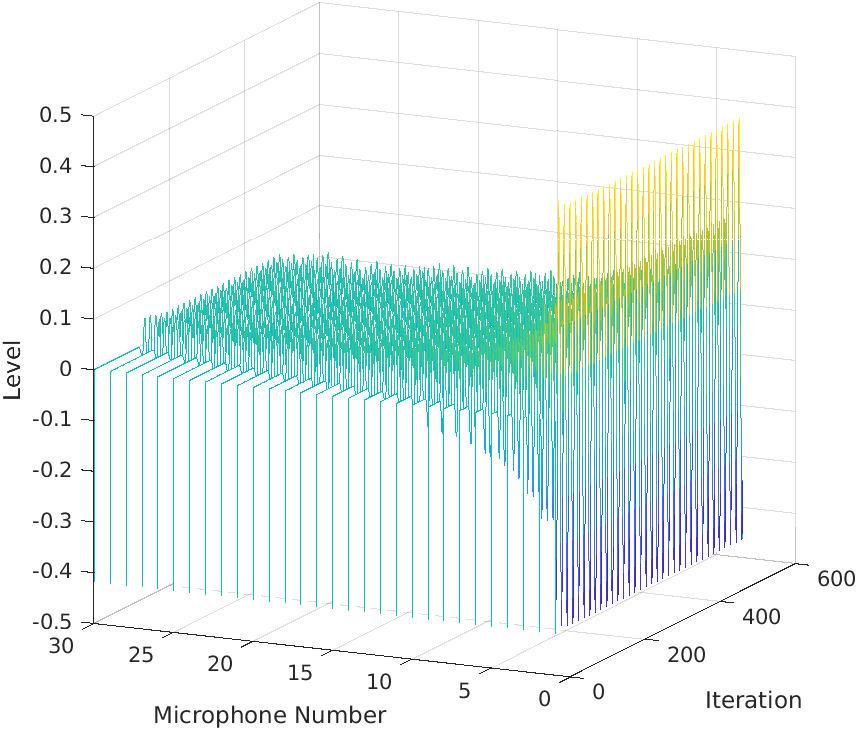
\includegraphics[width=75mm]{./Images/3_1_3d.png}
    \caption{3D graph of the received signals at the microphones}
    \label{fig_3_1_3D}
\end{figure}

With these signals we can calculate the sound pressure levels (SPLs) and plot
them against the distance, which is depicted in Fig. \ref{fig_3_1_spl}.
In the plot we can roughly see the expected $1/\sqrt{r}$ behavior of the
cylindrical spreading.

\begin{figure}[H]
    \centering
    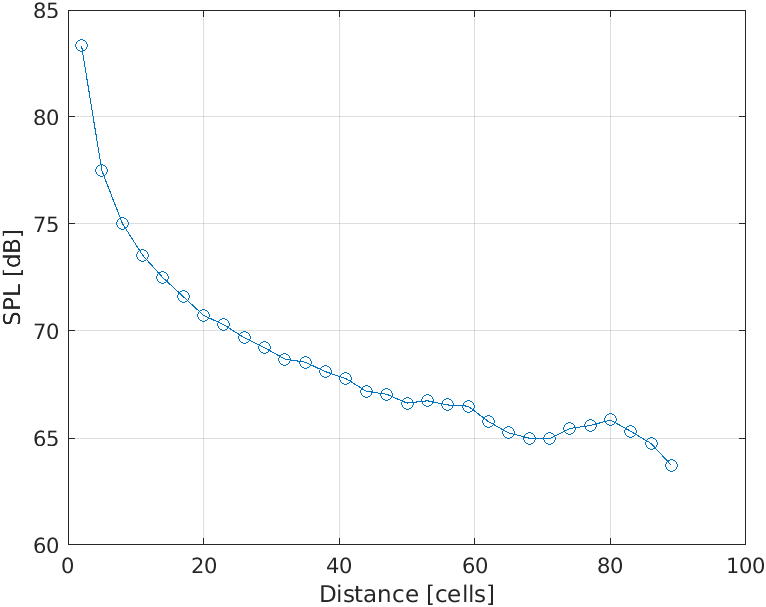
\includegraphics[width=75mm]{./Images/3_1_spls.png}
    \caption{The calculated SPLs for the microphone array against distance}
    \label{fig_3_1_spl}
\end{figure}

\subsection{Reflection from surface}
This next simulation is intended to study the behavior of the wave reflected from
surfaces with different reflection coefficient.
For this a surface was placed at the bottom in TLMfig.
The source was placed at $\left(50,59\right)$ and the 21 microphones were
placed at around the same height with the following coordinates
$\left(4n+10,60\right)$, where $n\in\left[0,20\right]$.

\begin{figure}[H]
    \centering
    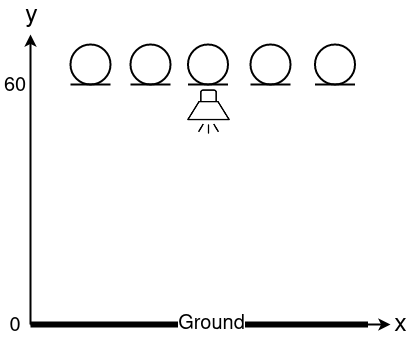
\includegraphics[width=55mm]{./Images/tlmfig_3_2.png}
    \caption{A depiction of the source and microphone arrangement to investigate reflection of surfaces}
    \label{fig_3_2_example}
\end{figure}


\subsection{Effect of noise screen}
The last simulation is intended to analyze the effect of a noise screen.
In this case the noise screen was simulated as a perfectly rigid wall.
The simulation configuration can be seen in Fig. \ref{fig_3_3_example}.
The ground has a reflection coefficient of $0.95$ and the source is set to noise with varying
number of cells per wavelength to achieve low- and high-frequency noise.

\begin{figure}[H]
    \centering
    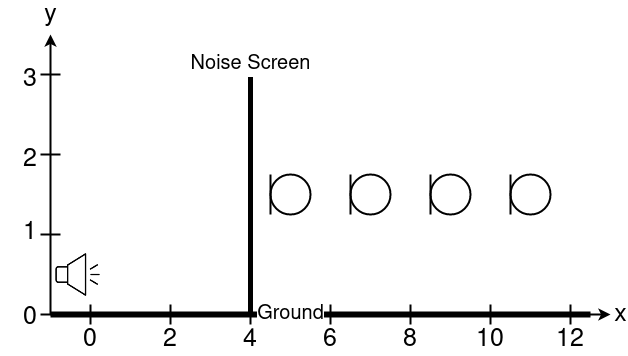
\includegraphics[width=75mm]{./Images/tlmfig_3_3.png}
    \caption{An exemplary setup of source and microphone for the noise screen simulation, with distances given in meters}
    \label{fig_3_3_example}
\end{figure}

The exact setup is given by the ground being at height of $10$ cells, the source at $\left(10,12\right)$, the
screen expands from $\left(18,10\right)$ to $\left(18,22\right)$, and the eleven microphones have the coordinates
$\left(4n+20,16\right)$ with $n\in\left[0,10\right]$.
To analyze the effect of the screen the simulation is run once with and once without screen.
\subsection{Discussion}

\section{Conclusion}

\subsection{Python}
\subsubsection{Matplotlib}
Using this library to plot the animation had some pitfalls.
The library uses a drawing buffer, which just fills over time.
Without manually clearing it before updating the plot, it will slow
the animation by a large amount.
Once that was introduced, a significant improvement could be observed.

\subsection{TLMfig}
While using this GUI some shortcomings were discovered.
Given that this might only be the case for the author's setup, which consisted
of a Linux machine without a dedicated GPU.

\subsubsection{Placing Objects}
Firstly, there are no coordinates for the cursor while drawing, which is only
a minor issue though.
If this was the case placing objects in the plane would be simplified a lot.
A workaround is drawing lines as helpers and erasing them to all but one pixel
at the edge of the plane.

\subsubsection{Exporting received signals}
Secondly, exporting the received data is not straightforward and this has some
overlap with the third problem.
Nevertheless possibilites could be to export the data which is plotted into the
Matlab workspace or generate a .mat file.
There's the option to export the configuration and grabbing the data from there,
but that's not exactly a logical step.

\subsubsection{Reusing stored configurations}
With talking about exporting the configuration we come to the third observation.
So assuming a configuration was saved and we reopen TLMfig.
Then try to open the stored configuration, it will open in a new TLMfig window.
This new window is solely a Matlab figure without the backend logic.
Therefore it cannot be used to re-run the stored configuration, making it impossible
to reproduce results without re-drawing the setup.

\subsubsection{GUI usage}
There are some additional behaviors that are unexpected.
E.g. the button label for placing mics updates to $1$ when a number is changed in the field,
then \textit{not} validated with the enter key, followed by clicking the button to place microphones.
It doesn't revert back and stays at the same number, which is $1$.

\begin{figure}[H]
    \centering
    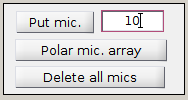
\includegraphics[width=45mm]{./Images/tlm_fig_button_label_good.png}
    \caption{TLMfig button label before bug}
\end{figure}
\begin{figure}[H]
    \centering
    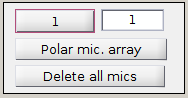
\includegraphics[width=45mm]{./Images/tlm_fig_button_label_bad.png}
    \caption{TLMfig button label after bug}
\end{figure}

Another unusual behavior is observed when using the input box to draw lines.
Sometimes one has to actually validate an input with the enter key and other times
it's enough to just change the value in the box and click somewhere else in the GUI
and a line is drawn.
This can lead to drawing way too many lines that were not intended if the user is not
aware of this.

\begin{figure}[H]
    \centering
    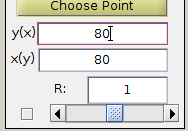
\includegraphics[width=45mm]{./Images/tlm_fig_updating_lines.png}
    \caption{Line drawing input box}
\end{figure}

\subsubsection{Final Words}
Even with all the beforementioned issues while using TLMfig, the GUI is largely helpful
for simulating wave propagation and analzying the behavior as reflections for example.


\section{References}

\small
\bibliographystyle{plain}
\bibliography{references}

\end{document}
